\begin{enumerate}
\item A ladder, leaning against a wall, makes an angle of $60 \degree$ with the horizontal.If the foot of the ladder is $2.5$ m away from the wall, find the length of the ladder.\\
\item  In \ref{figure_7}, a tent is in the shape of a cylinder surmounted by a conical top of same diameter. If the height and diameter of cylindrical part are $2.1$ m and $3$ m respectively and the slant height of conical part is $2.8$ m, find the cost of canvas needed to make the tent if the canvas is available at the rate of \rupee $500$/sq.metre.$\brak{\text{Use } \pi = \dfrac{22}{7}}$\\
	\begin{figure}[H]
      \centering
      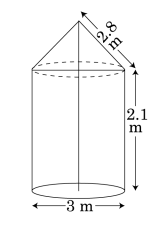
\includegraphics[width=5cm]{figs/2016_10_5.png}
      \caption{}
      \label{figure_7}
\end{figure} 
\item  In \ref{figure_8}, find the area of the shaded region, enclosed between two concentric circles of radii $7$ cm and $14$ cm where $\angle AOC = 40\degree$ $\brak{\text{Use }\pi =\dfrac{22}{7}}$.
	\begin{figure}[H]
      \centering
      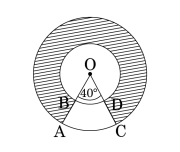
\includegraphics[width=5cm]{figs/2016_10_6.png}
      \caption{}
      \label{figure_8}
\end{figure} 
\item  A conical vessel, with base radius $5$ cm and height $24$ cm, is full of water. This water is emptied into a cylindrical vessel of base radius $10$ cm. Find the height to which the water will rise in the cylindrical vessel. $\brak{\text{Use } \pi  = \dfrac{22}{7}}$\\
\item  A sphere of diameter $12$ cm, is dropped in a right circular cylindrical vessel, partly filled with water. If a sphere is completely submerged in water, the water level in the cylindrical vessel rises by $ 3 \dfrac{5}{9}$cm. Find the diameter of the cylindrical vessel.\\  
\item  Due to heavy floods in a state, thousands were rendered homeless. $50$ schools collectively offered to the state government to provide place and the canvas for $1500$ tents to be fixed by the government and decided to share the whole expenditure equally. The lower part of each tent is cylindrical of base radius $2.8$ m and height $3.5$ m, with conical upper part of same base radius but of height $2.1$ m. If the canvas used to make the tents costs \rupee~120 per sq.m, find the amount shared by each school to set up the tents. What value is generated by the above problem ? (Use $ \pi = \dfrac{22}{7} ) $\\
\item  A man standing on the deck of a ship, which is $10$ m above water level, observes the angle of elevation of the top of a hill as $ 60\degree $ and the angle of depression of the base of hill as $ 30 \degree $. Find the distance of the hill from the ship and the height of the hill.\\
\item The angle of elevation of the top $Q$ of a vertical tower $PQ$ from a point $X$ on the ground is $ 60\degree $. From a point $Y$, $40$ m vertically above $X$, the angle of elevation of the top $Q$ of tower is $ 45 \degree $. Find the height of the tower $PQ$ and the distance $PX$. $\brak{\text{Use }\sqrt{3} = 1.73}$\\
\item A rectangular park is to be designed whose breadth is $3$ m less than its length.Its area is to be $4$ square metres more than the area of a park that has already been made in the shape of an isosceles triangle with its base as the breadth of the rectangular park and of altitude $12$ m. Find the length and breadth of the rectangular park.\\
\item In Fig  \ref{figure_9} , is shown a sector $OAP$ of a circle with centre $O$, containing $\angle \theta$. $AB$ is perpendicular to the radius $OA$ and meets $OP$ produced at $B$. Prove that the perimeter of shaded region is $r\sbrak{\tan \theta + \sec \theta + \dfrac{\pi \theta}{180}-1}$ \\

	\begin{figure}[H]
      \centering
      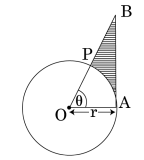
\includegraphics[width=5cm]{figs/2016_10_9.png}
     \caption{}
     \label{figure_9}
\end{figure} 
\end{enumerate}
